\documentclass{beamer}

%%% Работа с русским языком
\usepackage{cmap}					% поиск в PDF
\usepackage{mathtext} 				% русские буквы в формулах
\usepackage[T2A]{fontenc}			% кодировка
\usepackage[utf8]{inputenc}			% кодировка исходного текста
\usepackage[english,russian]{babel}	% локализация и переносы
\usepackage{indentfirst}
\frenchspacing

%%% Дополнительная работа с математикой
\usepackage{amsmath,amsfonts,amssymb,amsthm,mathtools} % AMS
\usepackage{icomma}

%%% Текст в колонки
\usepackage{multicol}

%%% Системы уравнений
\usepackage{cases}

%%% Таблицы
\usepackage{array}

%%% Картинки
\usepackage{graphicx}
\usepackage{float}

%%% Свои имена функций
\DeclareMathOperator{\Div}{div}
\DeclareMathOperator{\Const}{const}

%%% Список литературы
\usepackage[sorting=none]{biblatex}
\addbibresource{../references.bib}

%%% Гиперссылки
\usepackage{hyperref}

%%% Перенос знаков в формулах (по Львовскому)
\newcommand*{\hm}[1]{#1\nobreak\discretionary{}
{\hbox{$\mathsurround=0pt #1$}}{}}

%%% Цвета
\definecolor{red}{RGB}{200,0,0}


\usetheme{Madrid}
\title[Электрический пробой]{Моделирование электрического пробоя методом диффузной границы}
\author[]{
	Пономарев А.С.\textsuperscript{1,2},
	Савенков Е.Б.\textsuperscript{2},
	Зипунова Е.В.\textsuperscript{2}
}
\institute[]{
	\textsuperscript{1}МФТИ (НИУ) \\
	\textsuperscript{2}ИПМ им. М.В. Келдыша РАН
}
\date[]{
	66-я Всероссийская научная конференция МФТИ \\
	04.04.2024
}
\logo{
\includegraphics[height=0.8cm]{../figures/labels.jpg}}


\begin{document}

\AtBeginSection[]{
	\begin{frame}{Содержание}
	\Large
	\tableofcontents[currentsection]
	\end{frame}
}


\begin{frame}
\titlepage
\end{frame}


\begin{frame}{Содержание}
\Large
\tableofcontents
\end{frame}


\section{Введение}

\begin{frame}{Физическое явление}
\begin{block}{Электрический пробой}
	Явление резкого возрастания тока в диэлектрике при приложении электрического напряжения
	выше критического.
\end{block}
\begin{itemize}
	\item Рассматриваем твердый диэлектрик
	\item Деградация диэлектрических свойств материала
	\item Процесс развивается в ограниченной зоне -- канале
\end{itemize}
\end{frame}


\begin{frame}{Математическая модель}
\begin{block}{Модель типа диффузной границы}
	Вещество находится в разных фазах. Состояние вещества описывается гладкой функцией
	$\phi(\textbf{x}, t)$ -- фазовым полем.
\end{block}
\begin{itemize}
	\item $\phi = 1$ -- неповрежденная среда
	\item $\phi = 0$ -- полностью разрушенная среда
	\item Зона $\phi \in (0, 1)$ -- диффузная граница
	\item На разрушение среды тратится энергия
\end{itemize}
\begin{figure}
	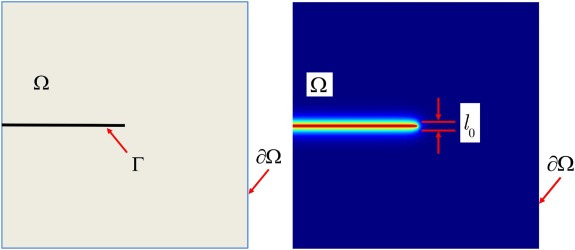
\includegraphics[width=0.6\textwidth]{../figures/diffuse_edge.jpg}
\end{figure}
\end{frame}


\begin{frame}{Математическая модель}
Модель, предложенная в работе \cite{kiam_model}:
\begin{itemize}
	\item $\pi = \textcolor{red}{-\cfrac{1}{2} \epsilon[\phi] (\nabla \Phi, \nabla \Phi)} +
	\Gamma \left( \cfrac{1 - f(\phi)}{l^2} + \cfrac{1}{4} (\nabla \phi, \nabla \phi) \right)$
	-- плотность свободной энергии
	\item $\Gamma$ -- энегрия роста пробоя на единицу длины
	\item $l$ -- величина <<размытия>> канала пробоя
	\item $\epsilon(\textbf{x}, t) = \cfrac{\epsilon_0(\textbf{x})}{f(\phi(\textbf{x}, t)) +
	\delta}$ -- диэлектрическая проницаемость среды
	\item $f(\phi) = 4 \phi^3 - 3 \phi^4$ -- интерполирующая функция
\end{itemize}
\end{frame}


\begin{frame}{Математическая модель}
\vspace{-0.5cm}
\begin{block}{Уравнения модели}
\begin{itemize}
	\item Уравнение электрического потенциала $\Phi$:
	\begin{equation}
		\Div(\epsilon[\phi] \nabla \Phi) = 0
		\label{equation_potential}
	\end{equation}
	\item Уравнение фазового поля $\phi$:
	\begin{equation}
		\cfrac{1}{m} \cfrac{\partial \phi}{\partial t} = \cfrac{1}{2} \epsilon'(\phi)
		(\nabla \Phi, \nabla \Phi) + \cfrac{\Gamma}{l^2} f'(\phi) +
		\cfrac{1}{2} \Gamma \triangle \phi
		\label{equation_phase}
	\end{equation}
\end{itemize}
\end{block}
Свойства:
\begin{itemize}
	\item связанная система уравнений на $\phi$ и $\Phi$;
	\item уравнение для $\phi$ типа Аллена--Кана, нелинейное.
\end{itemize}
\end{frame}


\begin{frame}{Пример вычислительного эксперимента}
\begin{columns}
\column{0.32\textwidth}
\begin{figure}
	
\includegraphics[width=\textwidth]{../figures/model_example_1.png}
\end{figure}
\column{0.32\textwidth}
\begin{figure}
	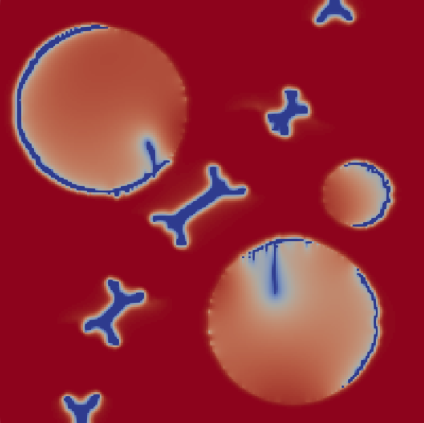
\includegraphics[width=\textwidth]{../figures/model_example_2.png}
\end{figure}
\column{0.32\textwidth}
\begin{figure}
	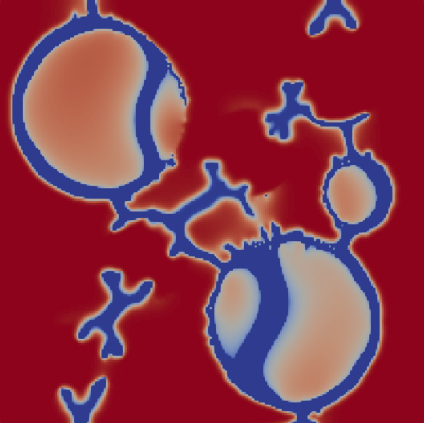
\includegraphics[width=\textwidth]{../figures/model_example_3.png}
\end{figure}
\end{columns}
\begin{center}
	Расчет из работы \cite{experiment_2d}
\end{center}
\end{frame}


\begin{frame}{Цель работы}
\begin{block}{Цель работы}
	Исследовать качественные характеристики системы уравнений \eqref{equation_potential},
	\eqref{equation_phase}: условия развития канала пробоя, границы применения разностной
	схемы.
\end{block}
Для этого будем рассматривать задачу в определенных краевых условиях, упрощающих ее, но
позволяющих установить интересующие нас свойства.
\end{frame}


\section{Постановка задачи}

\begin{frame}{Одномерная задача}
\vspace{-0.2cm}
\begin{itemize}
	\item Область $\Omega = [0, w]_x \times [0, h]_y \times I_z$ в форме параллелепипеда;
	\item $\phi(\textbf{x}, 0) = \phi_0(\textbf{x}) = \phi_0(x), \; \epsilon_0(\textbf{x}) =
	\epsilon_0(x)$ не зависят от $y$ и $z$;
	\item $\Phi|_{y = 0} = \Phi^- \in \mathbb{R}, \; \Phi|_{y = h} = \Phi^+ \in \mathbb{R}$.
\end{itemize}
\vspace{-0.5cm}
\begin{columns}
\column{0.5\textwidth}
Решением является функция электрического потенциала
\vspace{-0.2cm}
$$\Phi(\textbf{x}, t) = \Phi^- \hm + \cfrac{y}{h}(\Phi^+ - \Phi^-)$$
\column{0.5\textwidth}
\begin{figure}
	\vspace*{-0.3cm}
	\hspace*{0.5cm}
	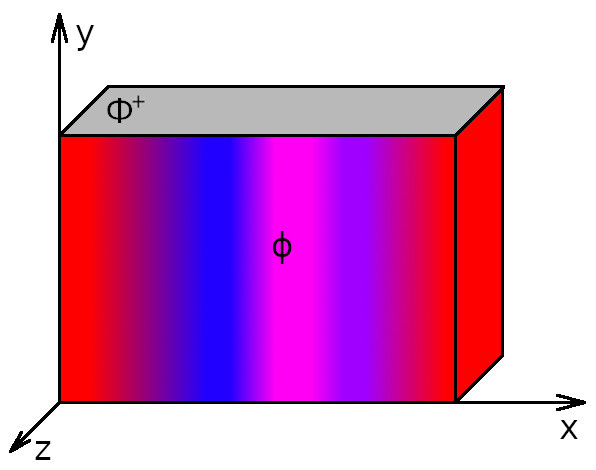
\includegraphics[width=0.7\textwidth]{../figures/one_dim_problem.jpg}
\end{figure}
\end{columns}
\vspace{-0.4cm}
Тогда уравнение на $\phi$ принимает вид
\begin{block}{}
	$$\cfrac{1}{m} \cfrac{\partial \phi}{\partial t} = \cfrac{1}{2} K_\Phi^2 \epsilon'(\phi) +
	\cfrac{\Gamma}{l^2} f'(\phi) + \cfrac{1}{2} \Gamma \cfrac{\partial^2 \phi}{\partial x^2}$$
\end{block}
$K_\Phi = \cfrac{\Phi^+ - \Phi^-}{h}$. Будем считать $\epsilon_0 = \Const$.
\end{frame}


\section{Теоретический анализ}

\begin{frame}{Анализ положений равновесия}
\begin{itemize}
	\item Пробой может развиваться из малых возмущений свойств неповрежденной среды. Выясним
	условия развития.
	\item Рассмотрим положения равновесия вида $\phi(x, t) \equiv C$. Положению равновесия
	соответствует ноль $C$ функции
\end{itemize}
$$\chi(\phi) = \cfrac{1}{2} K_\Phi^2 \epsilon'(\phi) + \cfrac{\Gamma}{l^2} f'(\phi)$$
\vspace{-0.5cm}
\begin{itemize}
	\item Исследуем положения равновесия на устойчивость спектральным методом: к $\phi \equiv C$
	прибавим возмущение $\delta \phi = e^{\alpha t}\cos(\omega x)$, линеаризуем уравнение на
	$\delta \phi$.
	\item $\chi(\phi)$ возрастает в $C \Longrightarrow$ равновесие неустойчиво; $\chi(\phi)$
	убывает в $C \Longrightarrow$ равновесие устойчиво.
\end{itemize}
\end{frame}


\begin{frame}{Анализ положений равновесия}
\vspace{-1cm}
\begin{columns}
\column{0.3\textwidth}
\begin{center}
	<<Слабое>> напряжение
\end{center}
$$0 \leqslant \cfrac{K_\Phi^2 l^2 \epsilon_0}{2 \Gamma} < \delta^2$$
\vspace{-0.3cm}
\begin{figure}
	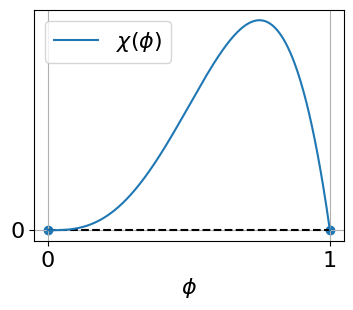
\includegraphics[width=\textwidth]{../figures/equilibriums_case_1.png}
\end{figure}
\column{0.3\textwidth}
\begin{center}
	<<Среднее>> напряжение
\end{center}
$$\delta^2 < \cfrac{K_\Phi^2 l^2 \epsilon_0}{2 \Gamma} < (1 + \delta)^2$$
\vspace{-0.3cm}
\begin{figure}
	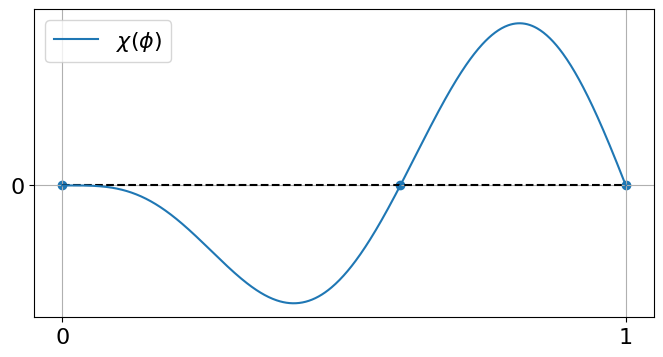
\includegraphics[width=\textwidth]{../figures/equilibriums_case_2.png}
\end{figure}
\column{0.3\textwidth}
\begin{center}
	<<Сильное>> напряжение
\end{center}
$$(1 + \delta)^2 < \cfrac{K_\Phi^2 l^2 \epsilon_0}{2 \Gamma}$$
\vspace{-0.3cm}
\begin{figure}
	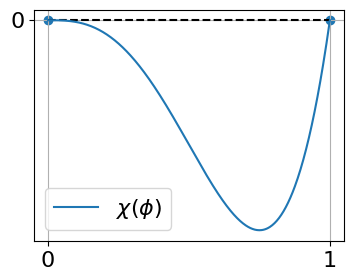
\includegraphics[width=\textwidth]{../figures/equilibriums_case_3.png}
\end{figure}
\end{columns}
\vspace{0.2cm}
\begin{columns}
\column{0.3\textwidth}
$\phi \equiv 0$ неустойчивое \\
$\phi \equiv 1$ устойчивое
\column{0.3\textwidth}
$\phi \equiv 0$ устойчивое \\
$\phi \equiv С_3$ неустойчивое \\
$\phi \equiv 1$ устойчивое
\column{0.3\textwidth}
$\phi \equiv 0$ устойчивое \\
$\phi \equiv 1$ неустойчивое
\end{columns}
\end{frame}


\section{Численный анализ}

\begin{frame}{Разностная схема}
\begin{block}{Разностная задача}
	$$\cfrac{1}{m} \cfrac{\phi_a^{b + 1} - \phi_a^b}{\tau} = \cfrac{1}{2} K_\phi^2
	\epsilon'(\phi_a^b) + \cfrac{\Gamma}{l^2} f'(\phi_a^b) + \cfrac{\Gamma}{2}
	\cfrac{\phi_{a + 1}^b - 2 \phi_a^b + \phi_{a - 1}^b}{h^2}$$
	$$\phi_a^0 = \phi_0(ah); \quad \phi_0^b = \phi_l(b \tau); \quad \phi_{w/h}^b = \phi_r(b \tau)$$
	Сетка регулярная; $\tau$ -- шаг по времени, $h$ -- шаг по пространству.
\end{block}
Явная разностная схема первого порядка по времени, второго -- по пространству.
\end{frame}


\begin{frame}{Оценка устойчивости}
\begin{itemize}
\item Рассмотрим возмущенное решение $\phi_a^b + \delta_a^b$. Линеаризуем уравнение на возмущение
$\delta_a^b$ в точке $\phi_a^b = P$:
\end{itemize}
$$\delta_a^{b + 1} = \delta_a^b + m \tau \left( \cfrac{1}{2} K_\Phi^2 \epsilon''(P) \delta_a^b +
\cfrac{\Gamma}{l^2} f''(P) \delta_a^b + \cfrac{\Gamma}{2} \cfrac{\delta_{a + 1}^b - 2 \delta_a^b +
\delta_{a - 1}^b}{h^2} \right)$$
\begin{itemize}
\item Применим спектральный признак устойчивости:
\end{itemize}
$$1 > \lambda(\theta) = 1 + m \tau \left( \cfrac{1}{2} K_\Phi^2 \epsilon''(P) +
\cfrac{\Gamma}{l^2} f''(P) - \cfrac{2 \Gamma}{h^2} \sin^2 \cfrac{\theta}{2} \right)$$
\begin{itemize}
\item Исследуем вблизи $P = 0$.
\end{itemize}
\end{frame}


\begin{frame}{Оценка устойчивости}
\begin{block}{Условие устойчивости}
	$$\tau \leqslant \cfrac{1}{2m \left( \cfrac{K_\Phi^2 \epsilon_0}{\delta^{5/3}} +
	\cfrac{\Gamma}{h^2} \right)}$$
\end{block}
\begin{block}{Упрощенное условие устойчивости}
	$$\tau \leqslant \cfrac{1}{4m} \min \left(\cfrac{\delta^{5/3}}{K_\Phi^2 \epsilon_0}, \;
	\cfrac{h^2}{\Gamma} \right)$$
\end{block}
\end{frame}


\begin{frame}{Вычисления: типичное решение}
\vspace{-0.4cm}
\begin{figure}
	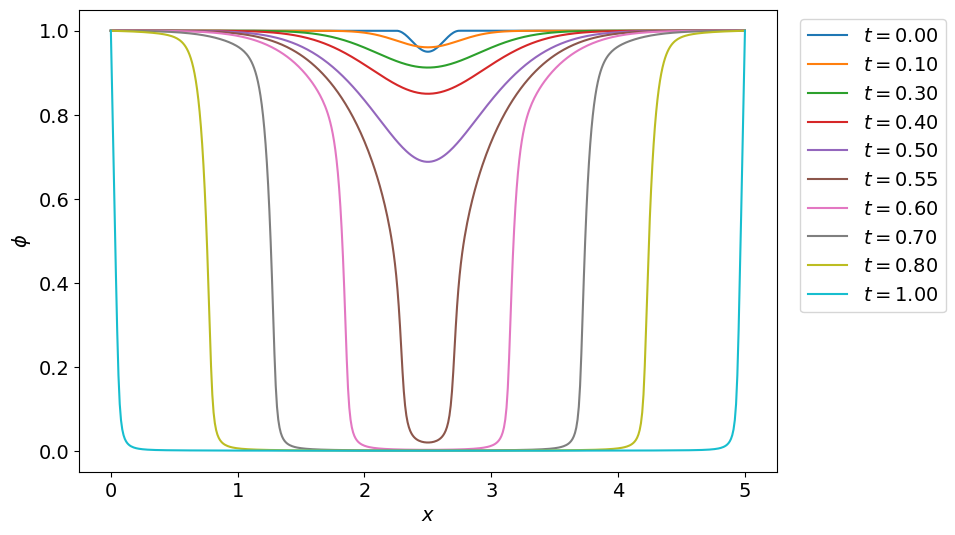
\includegraphics[width=\textwidth]{../figures/typical_solution.png}
\end{figure}
\vspace{-0.8cm}
\begin{center}
	Узлов по измерениям: $n_x = 10^3, \; n_t = 10^5$
\end{center}
\end{frame}


\begin{frame}{Вычисления: проверка устойчивости}
\vspace{-0.5cm}
\begin{figure}
	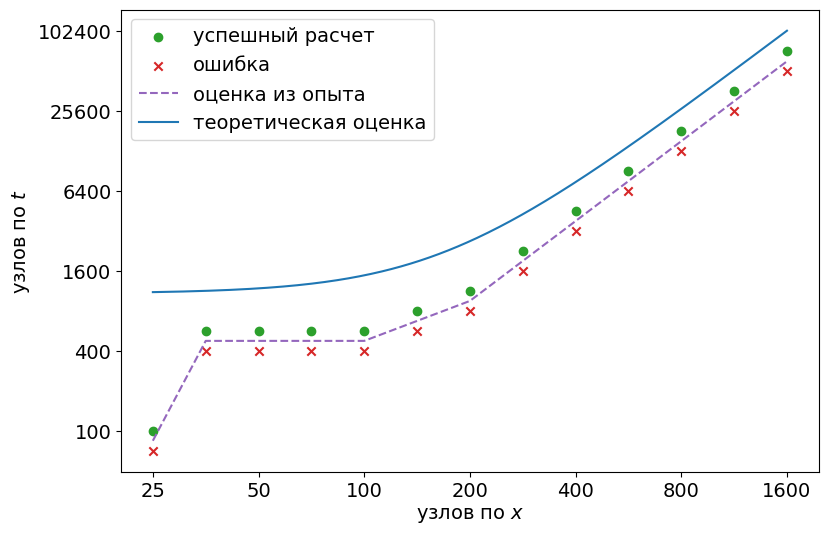
\includegraphics[width=0.75\textwidth]{../figures/stability_bounds.png}
\end{figure}
\vspace{-0.3cm}
$$\tau \leqslant \cfrac{1}{2m} \left( \cfrac{K_\Phi^2 \epsilon_0}{\delta^{5/3}} +
\cfrac{\Gamma}{h^2} \right)^{-1}$$
\end{frame}


\begin{frame}{Вычисления: проверка сходимости}
\vspace{-0.2cm}
\begin{figure}
	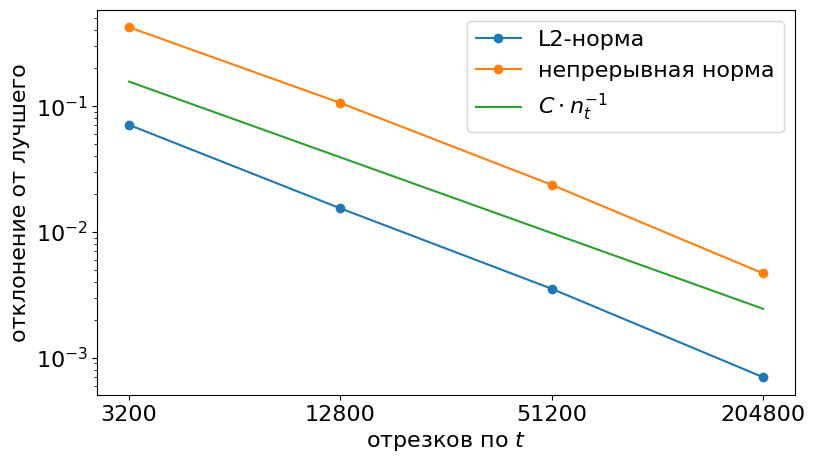
\includegraphics[width=0.75\textwidth]{../figures/convergence_connected.png}
\end{figure}
\vspace{-0.8cm}
\begin{center}
	\hspace{-0.4cm}
	Здесь, согласно оценке устойчивости, $\tau = \cfrac{h^2}{4m \Gamma}$
\end{center}
\end{frame}


\begin{frame}{Вычисления: положения равновесия}
\begin{center}
	$(1 + \delta)^2 < \cfrac{K_\Phi^2 l^2 \epsilon_0}{2 \Gamma}$ -- <<сильное>> напряжение
\end{center}
\begin{columns}
\column{0.45\textwidth}
\begin{figure}
	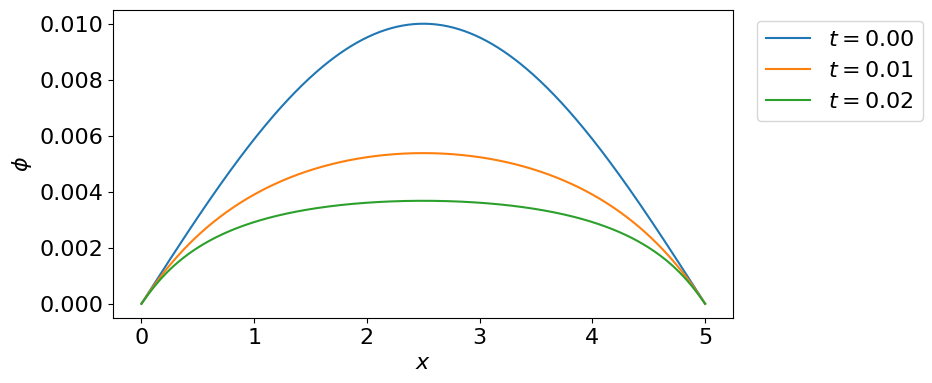
\includegraphics[width=\textwidth]{../figures/equilibrium_3_0.png}
\end{figure}
\begin{center}
	$\phi \equiv 0$ \\
	устойчивое
\end{center}
\column{0.45\textwidth}
\begin{figure}
	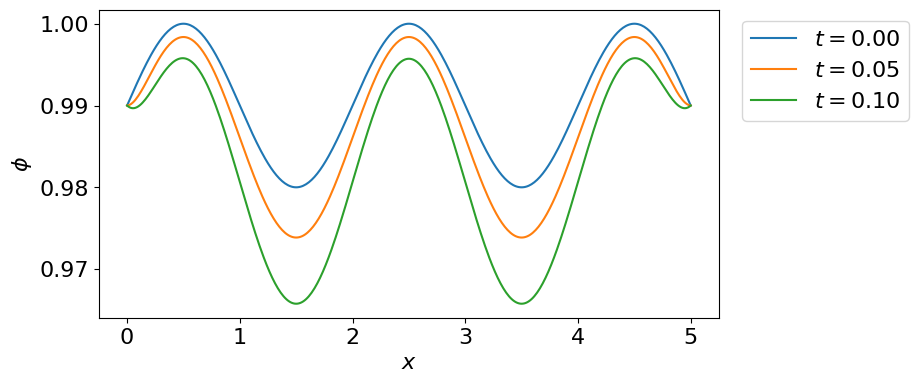
\includegraphics[width=\textwidth]{../figures/equilibrium_3_1.png}
\end{figure}
\begin{center}
	$\phi \equiv 1$ \\
	неустойчивое
\end{center}
\end{columns}
\end{frame}


\begin{frame}{Свободная энергия}
\vspace{-0.5cm}
$$\Pi(t) = \int\limits_\Omega \pi(x, t) dx$$
$$\pi(x, t) = \pi_1(x, t) + \pi_2(x, t) + \pi_3(x, t)$$
\vspace{-0.3cm}
\begin{itemize}
	\item $\pi_1(x, t) = -\cfrac{K_\Phi^2}{2} \, \epsilon(\phi(x, t))$ -- плотность энергии
	электрического поля;
	\item $\pi_2(x, t) = \Gamma \cfrac{1 - f(\phi(x, t))}{l^2}$ -- плотность энергии роста пробоя;
	\item $\pi_3(x, t) = \cfrac{\Gamma}{4} \left( \cfrac{\partial \phi}{\partial x}(x, t)
	\right)^2$ -- плотность энергии образования граничной зоны пробоя
\end{itemize}
\end{frame}


\begin{frame}{Вычисления: свободная энергия}
\vspace{-0.3cm}
\begin{columns}
\column{0.5\textwidth}
\begin{figure}
	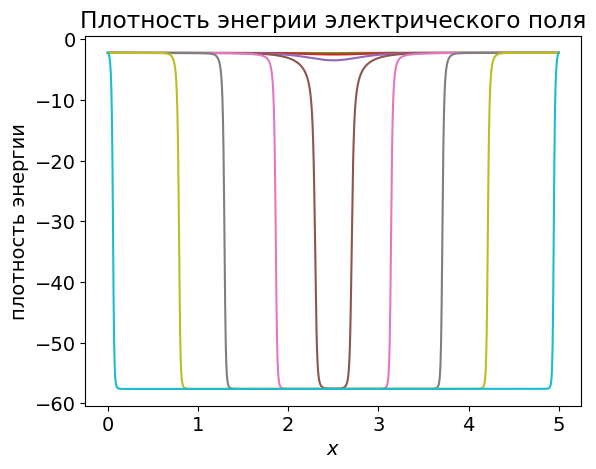
\includegraphics[width=0.75\textwidth]{../figures/density_electrical.png}
\end{figure}
\column{0.5\textwidth}
\begin{figure}
	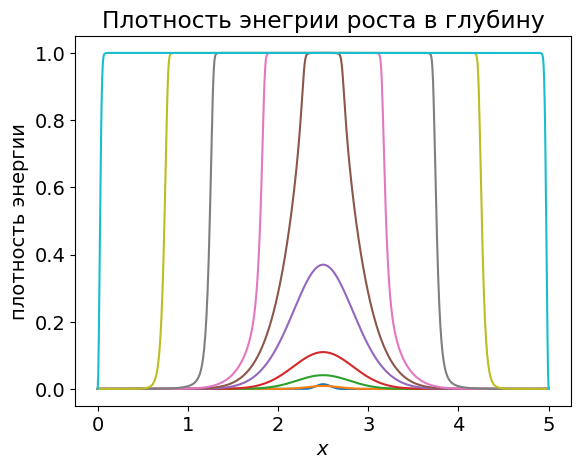
\includegraphics[width=0.75\textwidth]{../figures/density_depth.png}
\end{figure}
\end{columns}
\vspace{-0.3cm}
\begin{figure}
	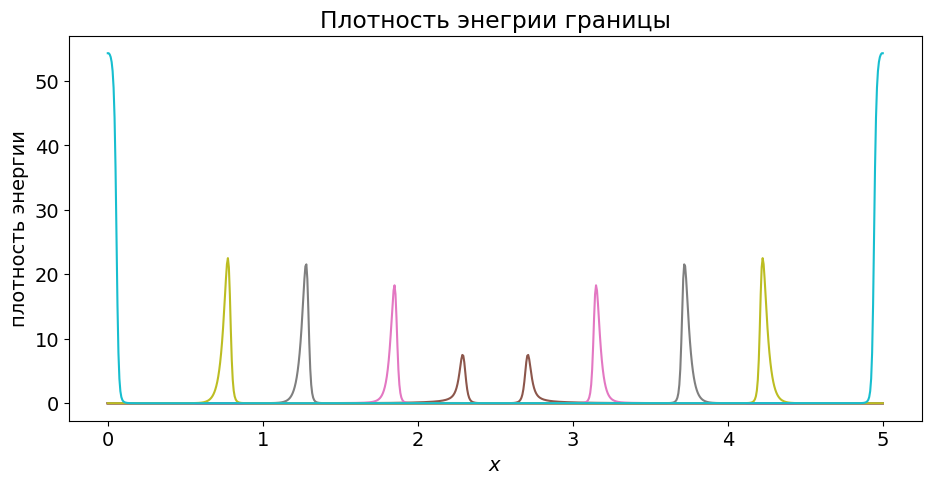
\includegraphics[width=0.65\textwidth]{../figures/density_surface.png}
\end{figure}
\end{frame}


\begin{frame}{Вычисления: свободная энергия}
\begin{figure}
	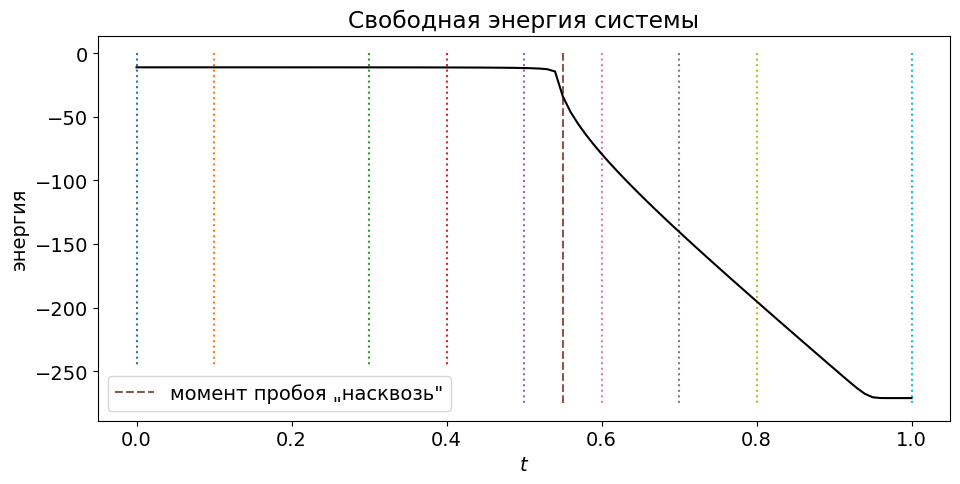
\includegraphics[width=\textwidth]{../figures/energy_total.png}
\end{figure}
\end{frame}


\begin{frame}{Литература}
\printbibliography
\end{frame}


\begin{frame}{}
\begin{center}
	\Large
	Спасибо за внимание
\end{center}
\end{frame}


\end{document}